\documentclass[12pt]{article}

\usepackage{graphicx}
\usepackage{paralist}
\usepackage{amsfonts}
\usepackage{hyperref}
\usepackage{listings}
\usepackage{subfig}

\oddsidemargin 0mm
\evensidemargin 0mm
\textwidth 160mm
\textheight 200mm
\renewcommand\baselinestretch{1.0}

\pagestyle {plain}
\pagenumbering{arabic}
\newcounter{stepnum}

\title{Course Project}
% \author{Hyosik Moon}
\author{
  Moon, Hyosik
  }

\begin {document}

\maketitle

\section{Required}

\begin{itemize}
\item \textbf{Main objective of the analysis} \\
Predict next-day rain by training classification models on the target variable RainTomorrow.

\item \textbf{Brief description of the data set} \\
This dataset contains about 10 years of daily weather observations from many locations across Australia.

RainTomorrow is the target variable to predict. It means -- did it rain the next day, Yes or No? This column is Yes if the rain for that day was 1mm or more.

In data set, there are 23 columns that 16 floats and 7 objects. \ref{data_info}

\begin{figure}[h!]
    \centering
    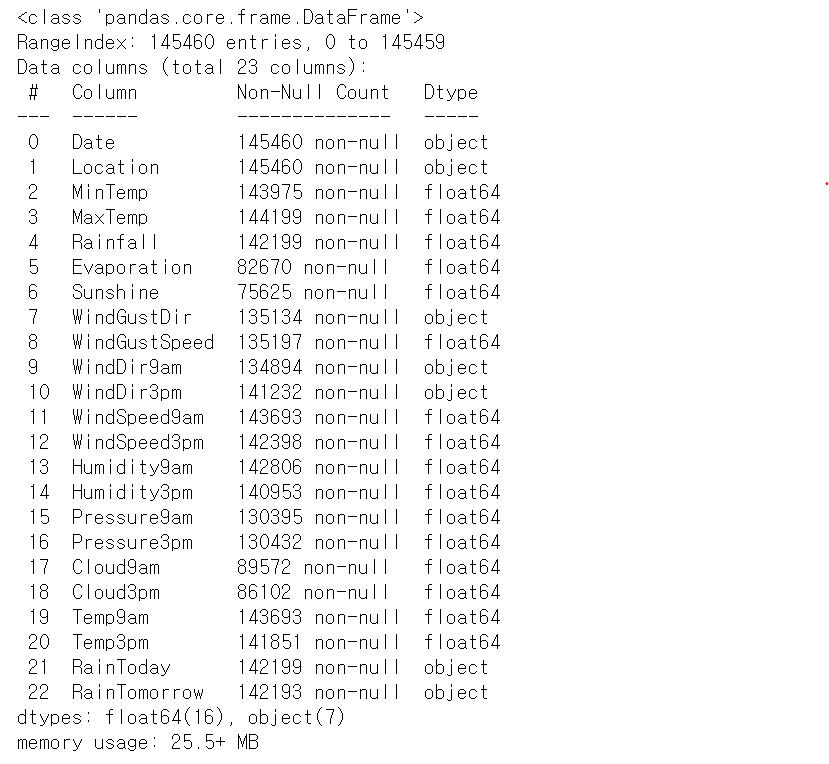
\includegraphics[width=0.9\textwidth]{figures/data_info.png}
    \caption{Data set information}\label{data_info}
\end{figure}

\item \textbf{Brief summary of data exploration}
    \begin{enumerate}
    \item Data cleaning, Delete unused features to predict the Ladder score. All data seem to be needed to predict the RainTomorrow, so before we check the correlation we won't delete any columns.
    \item In order to utilize Date columns, we need to change the type from object to int, and let's use just months for convenience.
    \item To see pairplot, we have to change categorical variables to numeric variables. So, let's change the objects to numeric by using LabelEncoder.
    \item Find the correlation between RainTomorrow and other features (Figure \ref{corr}). 
    
    \begin{figure}[h!]
      \centering
      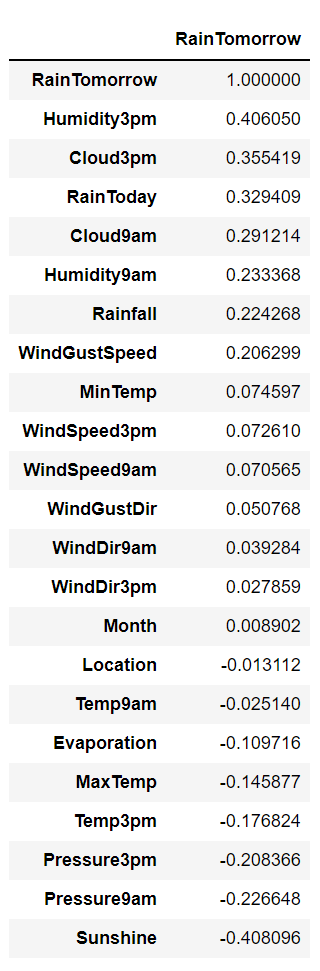
\includegraphics[width=0.3\textwidth]{figures/corr.png}
      \caption{Correlation}\label{corr}
    \end{figure}

    
    \item Change the categorical variable to numeric variables. (Figure \ref{ohc})
    
%     \begin{figure}[hbt!]
%         \centering
%         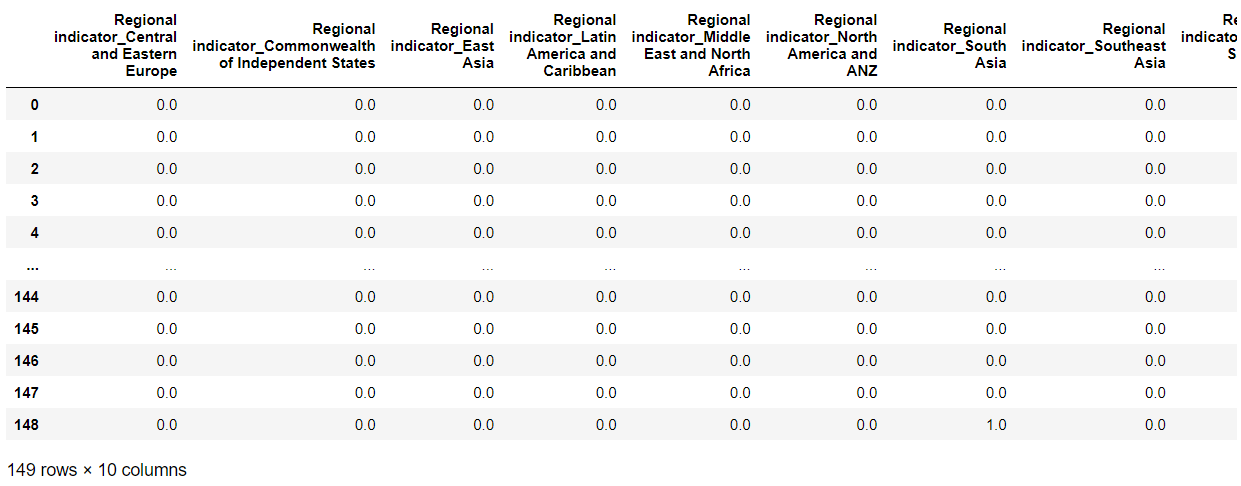
\includegraphics[width=0.8\textwidth]{figures/ohc.png}
%         \caption{OneHotEncoder}\label{ohc}
%     \end{figure}

%     \item Standardize the features. (Figure \ref{std})

%     \begin{figure}[hbt!]
%         \centering
%         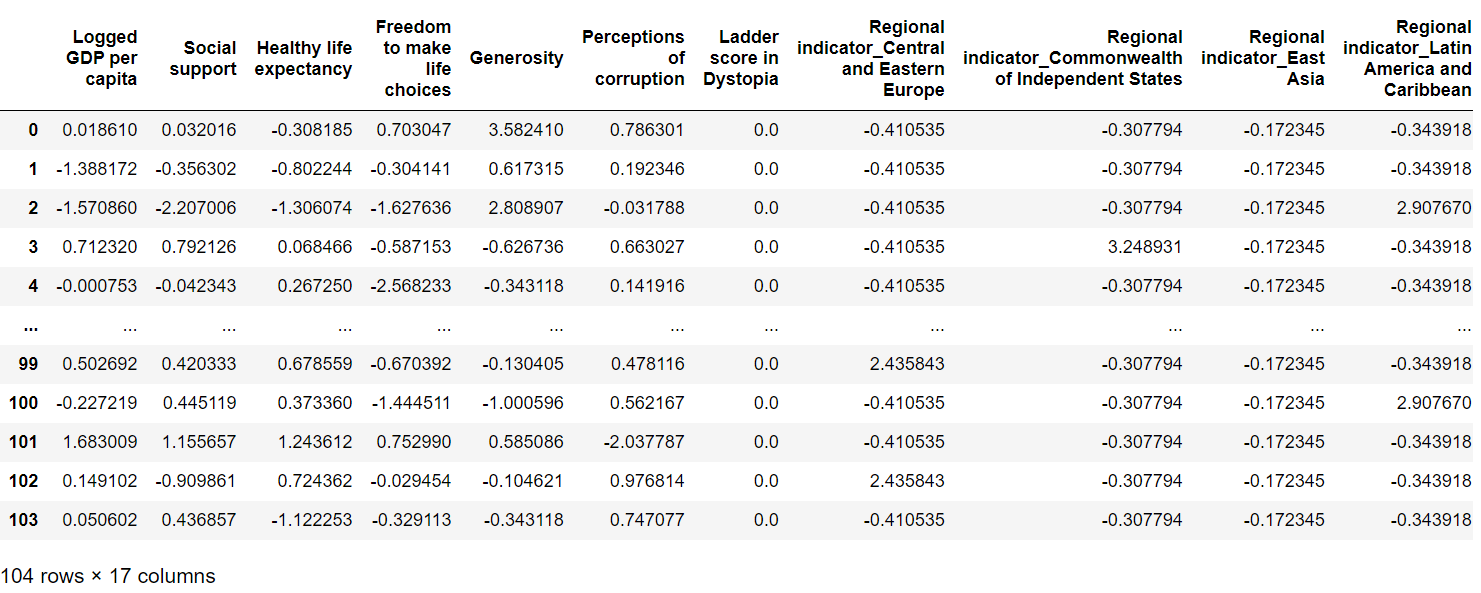
\includegraphics[width=0.8\textwidth]{figures/std.png}
%         \caption{Standardized values}\label{std}
%     \end{figure}

%     \item Check the normality of the target value and normalize if it's skewed. \\
%     \textit{Ladder score}'s p-value is 0.526. So, we don't need to normalize the target value. (Figure \ref{nom})

%     \begin{figure}[hbt!]
%         \centering
%         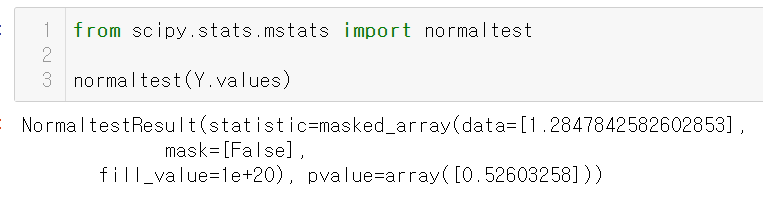
\includegraphics[width=0.8\textwidth]{figures/normalize.png}
%         \caption{Check the normality of the target}\label{nom}
%     \end{figure}
    
    \end{enumerate}

\item \textbf{Summary of training at least three linear regression models}
% We tested 4 kinds of models such as \textit{Linear Regression, Lasso, Ridge, ElasticNet} and in order to prevent overfitting we used cross validation. To evalueate the best model, we compare the results with rmse(root mean squared error). This is the result of rmse of the four models. (Figure \ref{rmse})

% \begin{figure}[hbt!]
%     \centering
%     \includegraphics[width=0.4\textwidth]{figures/rmse.png}
%     \caption{Check the rmse of the models}\label{rmse}
% \end{figure}

\item \textbf{Explanation of your final regressions model}
% Overall, all models showed the low rmse values. But the best one was Ridge $(ridgeCV.alpha\_ :  21.056578947368422  ridgeCV\_rmse:  0.501828479703691)$. And the r2\_score of the model was $0.7610082843481112$.

\item \textbf{Summary Key Findings and Insights}
% When we analyze the coefficients, it shows the interesting result. The regions are the main fators that people feel happy. I think it's resonable because happiness is decided based on the relationship. So, some regions might have a culture that put big emphasis on the relationship (Figure \ref{factors})

% \begin{figure}[hbt!]
%     \centering
%     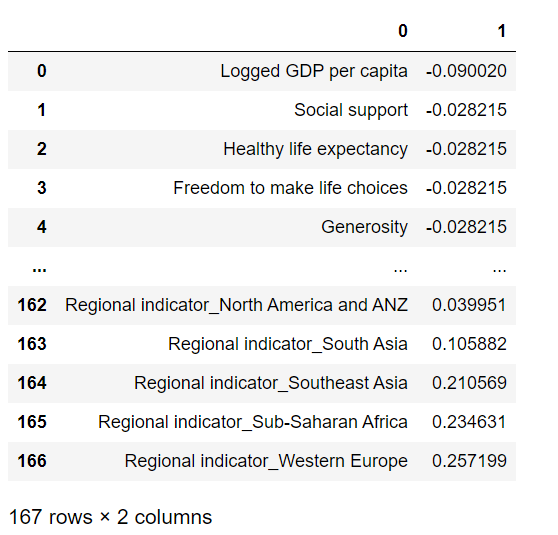
\includegraphics[width=0.8\textwidth]{figures/factors.png}
%     \caption{Coefficients. Regions are the main factors}\label{factors}
% \end{figure}

\item \textbf{Suggestions for next steps}
% We may find more meaningful results if we exclude the regions to predict the target. Because regions can be the result of different features such as GDP, Healthy, Social support, etc. Then, we will know the factor that has the most impact on the happiness rather than the regions.

\end{itemize}

\end {document}